\subsection{Focusing on Specific Desired Properties with Reinforcement Learning}
\label{subsec:rel-unsup-specific-properties}
\begin{figure}[ht]
    \centering
    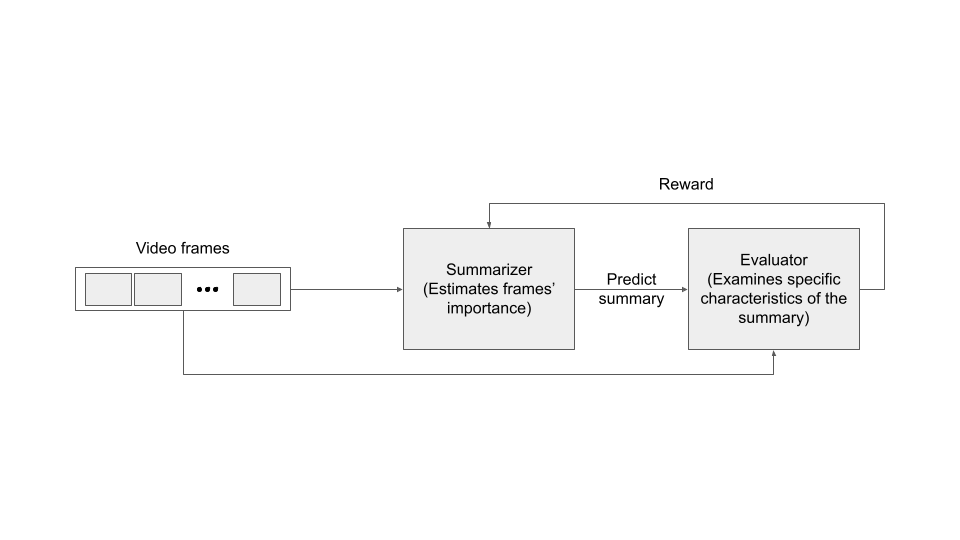
\includegraphics[width=0.73\paperwidth]{content/related/figures/unsup-characteristics.png}
    \caption{High-level representation of the analysis pipeline of supervised algorithms that learn summarization based on hand-crafted rewards and reinforcement learning.}
    \label{figure:rel-unsup-properties}
  \end{figure}

Addressing the challenges of unstable training and limited evaluation criteria in GAN-based methods, certain unsupervised approaches focus on specific properties of an optimal video summary. These approaches employ reinforcement learning principles in conjunction with hand-crafted reward functions that quantify desired characteristics in the generated summary. Illustrated in \hyperref[figure:rel-unsup-properties]{Figure \ref{figure:rel-unsup-properties}}, the Summarizer takes the video frame sequence as input and generates a summary by predicting frame-level importance scores. The predicted summary is then evaluated by an Evaluator, which employs hand-crafted reward functions to measure the presence of specific desired characteristics. The computed scores are combined to form an overall reward value, guiding the training of the Summarizer.

The initial work in this direction, proposed by Zhou \etal~\cite{zhou2018deep}, formulates video summarization as a sequential decision-making process. They train a Summarizer to produce diverse and representative video summaries using a diversity-representativeness reward. The diversity reward quantifies the dissimilarity among selected keyframes, while the representativeness reward measures the visual resemblance of the selected keyframes to the remaining frames of the video. Expanding on this method, Yaliniz \etal~\cite{yaliniz2021using} present another reinforcement-learning-based approach that incorporates the uniformity of the generated summary. They employ Independently Recurrent Neural Networks (IndRNNs) activated by a Leaky ReLU function to model temporal dependencies among frames. This addresses issues related to decaying, vanishing, and exploding gradients in LSTM models and facilitates better learning of long-term dependencies. In addition to rewards associated with representativeness and diversity, Yaliniz et al. introduce a uniformity reward to enhance the coherence of the summary and prevent redundant jumps between selected video fragments. Gonuguntla \etal~\cite{gonuguntla2019enhanced} propose a method utilizing Temporal Segment Networks, originally designed for action recognition in videos, to extract spatial and temporal information from video frames. They train the Summarizer using a reward function that evaluates the preservation of the video's main spatiotemporal patterns in the generated summary. Lastly, Zhao \etal~\cite{zhao2019property}present a mechanism that combines video summarization and reconstruction. Video reconstruction aims to estimate how well the summary allows viewers to infer the original video, similar to some GAN-based methods. Video summarization is learned based on feedback from the reconstructor and the output of trained models that assess the representativeness and diversity of the visual content in the generated summary.

In conclusion, reinforcement learning has emerged as a promising alternative to GAN-based methods in the field of video summarization. By employing principles of sequential decision-making and custom reward functions, these techniques strive to produce video summaries that are diverse, representative, and coherent. This approach overcomes the challenges of training stability and limited evaluation criteria often associated with GAN-based approaches. By incorporating rewards for diversity, representativeness, uniformity, and preservation of spatiotemporal patterns, the Summarizer can effectively learn optimal summary generation. Although still a developing area, reinforcement learning in video summarization shows great potential for advancing the development of automated summarization algorithms that effectively capture key information while preserving the visual integrity of the original videos. Ongoing research and experimentation will undoubtedly refine and enhance the capabilities of reinforcement learning-based approaches in this domain.